\documentclass[12pt, titlepage, oneside]{article}

\usepackage[margin=0.5in]{geometry}

\usepackage{siunitx, booktabs, amsmath, enumitem, pdfpages,mathrsfs,tabularx,caption, graphicx, pgfplots, textcomp,wrapfig, commath, svg}

\usepackage{amssymb}

\usepackage{parskip}

\usepackage[siunitx]{circuitikz}
\sisetup{detect-weight=true, detect-family=true}

\setlength\parindent{0pt}

\let\oldhat\hat
\let\oldvec\vec
\newcommand{\cross}{\bm{\times}}
\renewcommand{\hat}[1]{\oldhat{\mathbf{#1}}}

\usepackage{bm}
\renewcommand{\vec}[1]{\oldvec{\bm{#1}}}
\renewcommand{\hat}[1]{\oldhat{\bm{#1}}}
\renewcommand{\b}[1]{\textbf{#1}}

\newcommand{\de}[1]{\noindent\fbox{\parbox{\textwidth}{#1}}}

\newcommand{\be}{\begin{equation*}}
\newcommand{\ee}{\end{equation*}}

\begin{document}
	\setcounter{section}{7}
	\setcounter{page}{22}

    \section{Continuous Random Variable }

    \b{Continuous random variables} are variables that arise from measurements that can take any value within intervals.

    Recall that p.m.f $f(x)$ can be represented by masses at discrete points on a real line. For continuous random variables, these masses are smeared continuously between discrete points. Thus giving rise to a density function as we try to describe the mass per unit length on the $x$-axis, we call this distribution a \b{probability density function(p.d.f)} $f(x)$. The p.d.f describes probability of a continuous random variable $X$.

    For a continuous random variable $X$, a probability density function is a function such that
    \begin{enumerate}
      \item $f(x) \geq 0$ : The probability density function is always greater than or equal to zero.
      \item $\int_{-\infty}^{+\infty} f(x) dx = 1$ : The total area under the graph of $f(x) = 1$

      The area under $f(x)$ on any interval equals the true probability that a measurements falls in the interval.

      \item $P(a \leq X \leq b) = \int_a^b f(x) dx = $ area under $f(x)$ from $a$ to $b$ for any $a,b$

      \item $P(X = x) = 0$ :  Since there is no area defined, no measurement falls in an infinitely small range
    \end{enumerate}

          \begin{center}
        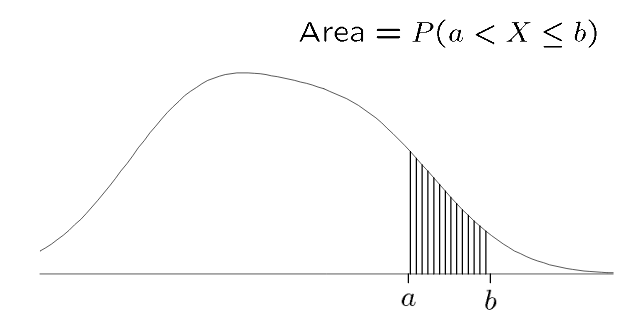
\includegraphics[scale=0.5]{1.png}
       \end{center}
    
    \de{
      \b{Example 4.2 } Hole diameter $X$ has p.d.f
      \begin{align*}
        f(x) = \begin{cases} 20e^{-20(x-12.5)} & x \geq 12.5 \\ 0 & \text{else} \end{cases}
        \end{align*}
        Find $P(X > 12.60)$ and $P(12.5 < X < 12.6)$
        \\
        
        \b{Ans.}
        \begin{align*}
          P(X > 12.60 ) = \int_{12.60}^{\infty}f(x)dx = \int_{12.60}^{\infty} 20e^{-20(x-12.5)} dx = -e^{-20(x-12.5)}|_{12.6}^{\infty} = 0.135\\[2mm]
          P(12.5 < X < 12.6) = \int_{12.50}^{12.60}f(x)dx = \int_{12.50}^{12.60}20e^{-20(x-12.5)}dx = -e^{-20(x-12.5)}|_{12.5}^{12.6} = 0.865
        \end{align*}
              \begin{center}
       \end{center}
    }
    
\end{document}